\documentclass{article}
\usepackage[utf8x]{inputenc}
\usepackage{ucs}
\usepackage{amsmath} 
\usepackage{amsfonts}
\usepackage{marvosym}
\usepackage{wasysym}
\usepackage{upgreek}
\usepackage[english,russian]{babel}
\usepackage{graphicx}
\usepackage{float}
\usepackage{textcomp}
\usepackage{hyperref}
\usepackage{geometry}
  \geometry{left=2cm}
  \geometry{right=1.5cm}
  \geometry{top=1cm}
  \geometry{bottom=2cm}
\usepackage{tikz}
\usepackage{ccaption}
\usepackage{multicol}

\hypersetup{
   colorlinks=true,
   citecolor=blue,
   linkcolor=black,
   urlcolor=blue
}

\usepackage{listings}
%\setlength{\columnsep}{1.5cm}
%\setlength{\columnseprule}{0.2pt}

\usepackage[absolute]{textpos}

\usepackage{colortbl,graphicx,tikz}
\definecolor{X}{rgb}{.5,.5,.5}


\begin{document}
\pagenumbering{gobble}
\lstset{
  language=C,                % choose the language of the code
  basicstyle=\linespread{1.1}\ttfamily,
  columns=fixed,
  fontadjust=true,
  basewidth=0.5em,
  keywordstyle=\color{blue}\bfseries,
  commentstyle=\color{gray},
  stringstyle=\ttfamily\color{orange!50!black},
  showstringspaces=false,
  numbersep=5pt,
  numberstyle=\tiny\color{black},
  numberfirstline=true,
  stepnumber=1,                   % the step between two line-numbers.        
  numbersep=10pt,                  % how far the line-numbers are from the code
  backgroundcolor=\color{white},  % choose the background color. You must add \usepackage{color}
  showstringspaces=false,         % underline spaces within strings
  captionpos=b,                   % sets the caption-position to bottom
  breaklines=true,                % sets automatic line breaking
  breakatwhitespace=true,         % sets if automatic breaks should only happen at whitespace
  xleftmargin=.2in,
  extendedchars=\true,
  keepspaces = true,
}
\lstset{literate=%
   *{0}{{{\color{red!20!violet}0}}}1
    {1}{{{\color{red!20!violet}1}}}1
    {2}{{{\color{red!20!violet}2}}}1
    {3}{{{\color{red!20!violet}3}}}1
    {4}{{{\color{red!20!violet}4}}}1
    {5}{{{\color{red!20!violet}5}}}1
    {6}{{{\color{red!20!violet}6}}}1
    {7}{{{\color{red!20!violet}7}}}1
    {8}{{{\color{red!20!violet}8}}}1
    {9}{{{\color{red!20!violet}9}}}1
}

\title{Семинар \#8: Стек и Очередь. Домашнее задание.\vspace{-5ex}}\date{}\maketitle

\section*{Абстрактные типы данных: Стек, очередь, дек, очередь с приоритетом}
\quad

\textbf{Абстракстный тип данных (АТД)} - это математическая модель для типов данных, которая задаёт поведение этих типов, но не их внутреннею реализацию.\\

\textbf{Стек (Stack)} - это АТД, который представляет собой коллекцию элементов, менять которые можно только с помощью двух операций:
\begin{itemize}
\item \texttt{push} - добавить элемент в стек.
\item \texttt{pop} - извлечь из стека последний добавленный элемент.
\end{itemize}
Таким образом, поведение стека задаётся этими двумя операциями. Так как стек - это абстрактный тип данных, то его внутренняя реализация на языке программирования может быть самой разной. Стек можно сделать на основе статического массива, на основе динамического массива(\texttt{malloc}/\texttt{free}) или на основе связного списка. Внутренняя реализация не важна, важно только наличие операций \texttt{push} и \texttt{pop}. \\
Не нужно путать абстракстный тип данных стек с сегментом памяти стек.\\

\textbf{Очередь (Queue)} - это АТД, который представляет собой коллекцию элементов, менять которые можно только с помощью двух операций:
\begin{itemize}
\item \texttt{enqueue} - добавить элемент в очередь.
\item \texttt{dequeue} - извлечь из очереди первый добавленный элемент из оставшихся.
\end{itemize}

\begin{center}
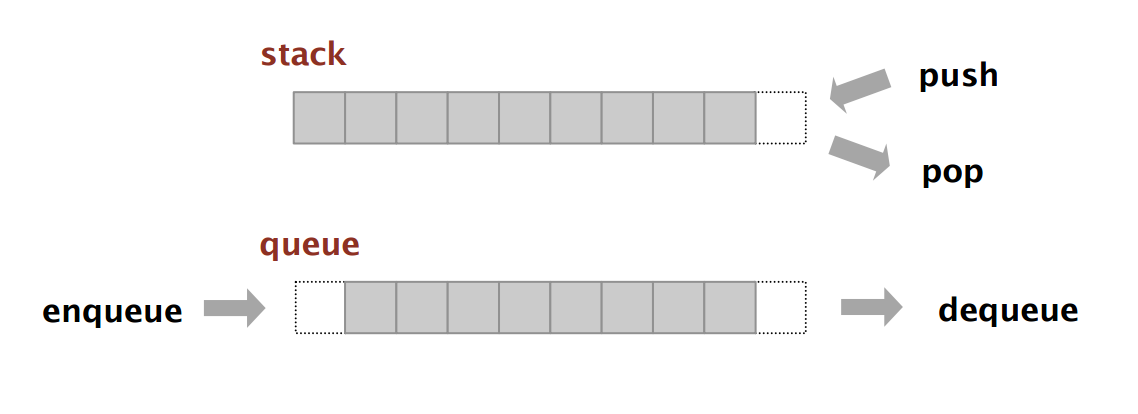
\includegraphics[scale=0.31]{../images/stack_queue.png}
\end{center}

\textbf{Дек (Deque = Double-ended queue)} - это АТД, который представляет собой коллекцию элементов, менять которые можно только с помощью четырёх операций:
\begin{itemize}
\item \texttt{push\_back} - добавить элемент в конец.
\item \texttt{push\_front} - добавить элемент в начало.
\item \texttt{pop\_back} - извлечь элемент с конца.
\item \texttt{pop\_front} - извлечь элемент с начала.\\
\end{itemize}

\textbf{Очередь с приоритетом (Priority Queue)} - это АТД, который представляет собой коллекцию элементов, менять которые можно только с помощью двух операций:
\begin{itemize}
\item \texttt{insert} - добавить элемент.
\item \texttt{extract\_best} - извлечь из очереди элемент с наибольшим приоритетом. 
\end{itemize}
То, что будет являться приоритетом может различаться. Это может быть как сам элемент, часть элемента (например, одно из полей структуры) или другие данные, подаваемые на вход операции \texttt{insert} вместе с элементом. В простейшем случае, приоритетом является сам элемент (тогда очередь с приоритетом просто возвращает максимальный элемент) или сам элемент со знаком минус (тогда очередь с приоритетом возвращает минимальный элемент).

\section*{Реализация стека на основе статического массива}
В файле \texttt{stack/1stack.c} представлена реализация стека на основе статического массива.\\ 
Основные моменты такой реализации:
\begin{itemize}
\item Константа \texttt{CAPACITY} задаёт вместимость стека. Эта величина будет постоянна во время выполнения программы. Если, вдруг, во время выполнения программы нам понадобится больше места в стеке, то мы ничего сделать не сможем и придётся писать сообщение об ошибке и завершать программу. В то же время, если в этом стеке будет мало элементов, то он всё-равно будет потреблять память соответствующую \texttt{CAPACITY} элементам. Эти недостатки решаются в реализации на основе динамического массива.
\item Строка 
\begin{lstlisting}
typedef int Data;
\end{lstlisting}
создаёт новое имя для типа \texttt{int}. Благодаря этому вместо \texttt{int} можно писать \texttt{Data}. Это нужно для того, чтобы можно было легко менять тип элемента, который хранит стек. Если, например, мы захотим хранить в стеке не \texttt{int}-ы, а \texttt{char}-ы или что-то другое, то мы просто изменим эту строку. Однако, если нам понадобится в одной программе использовать 2 стека с разными типами, то такое не пройдёт и нам придётся дублировать код для разных стеков. От этого недостатка можно избавиться в языке \texttt{C++} с помощью шаблонов.
\item Структура \texttt{Stack} содержит целое \texttt{size} -- количество элементов в стеке и массив \texttt{values} - массив размера \texttt{CAPACITY}, в первых \texttt{size} ячейках которого будут хранится элементы стека.
\item Функция \texttt{stack\_init} задаёт поля структуры стека для начала работы с ним. В данном случае она просто зануляет \texttt{n}. В других реализациях аналогичные функции будут иметь более сложный вид.
\item Функция \texttt{stack\_push} добавляет элемент \texttt{x} в стек. Если стек уже заполнен, то программа завершает своё выполнение с ошибкой. Стек передаётся по указателю, так как он будет меняться внутри функции.
\item Функция \texttt{stack\_pop} удаляет последний элемент стека и возвращает его. Если стек пуст, то программа завершает своё выполнение с ошибкой.
\item Функция \texttt{stack\_get} возвращает последний элемент стека. Стек передаётся по \texttt{const}-указателю, так как стек не будет меняться внутри этой функции. А передавать стек в функцию по значению было бы слишком затратно, так как происходило бы копирование всего стека.
\end{itemize}

\newpage
\section*{Реализация стека на основе динамического массива}
В файле \texttt{stack/2stack\_dynamic.c} представлена реализация стека на основе динамического массива.\\ 
Основные моменты такой реализации:
\begin{itemize}
\item Структура \texttt{Stack} содержит \texttt{capacity} -- вместимость стека, \texttt{size} -- количество элементов в стеке и указатель \texttt{values}. Указатель \texttt{values} будет указывать на участок памяти, выделенной с помощью \texttt{malloc}. Размеры выделенной памяти будут храниться в поле \texttt{capacity}.
\item Функция \texttt{stack\_init} теперь должна задать \texttt{size} и \texttt{capacity}, а также выделить начальную область памяти под стек. Код выделения
памяти выглядит следующим образом:
\begin{lstlisting}
s->values = (Data*)malloc(s->capacity * sizeof(Data));
if (s->values == NULL)
{
	printf("Error! Could not allocate memory.\n");
	exit(1);
}
\end{lstlisting}
В первой строке мы пытаемся выделить необходимое количество памяти. При этом иногда (очень редко) у \texttt{malloc}-а может не получиться выделить нужное количество памяти (например если вся память кончилась). В этом случае \texttt{malloc} возращает \texttt{NULL}. Если это происходит, то мы должны завешить программу.
\item Функция \texttt{stack\_push} добавляет элемент в стек. Но перед тем, как это сделать функция проверит, если в стеке место. Если места нет, то функция должна увеличить вместимость динамического массива. Происходит это следующим образом:
\begin{lstlisting}
s->capacity *= 2;
Data* temp = (Data*)realloc(s->values, s->capacity * sizeof(int));
if (temp == NULL)
{
	printf("Error! Could not reallocate memory\n");
	free(s->values);
	exit(1);
}
else
{
	s->values = temp;
}
\end{lstlisting}
В второй строке мы пытаемся выделить больше памяти. Если перевыделение прошло успешно, то указатель \texttt{temp} будет хранить адрес новой памяти. При этом старая память автоматически освободится. Если же перевыделение не сработало(память кончилась), то \texttt{temp} будет равным \texttt{NULL}.
\end{itemize}

\section*{Задачи}
\textbf{Задача \#1: Размер и вместимость}:
Напишите программу, которая будет создавать стек(динамический) вместимости \texttt{7} и добавлять в него последовательно \texttt{200} элементов. При каждом добавлении элемента печатайте размер и вместимость стека.\\
\textbf{Задача \#2: Скобочки}: Написать программу которая будет считывать последовательность скобочек и
печатать \texttt{Yes} или \texttt{No} в зависимости от того является ли эта последовательность допустимой.  Используйте одну из реализаций стека. Для считывания строки: \texttt{scanf(``\%s'', str);}
\begin{multicols}{2}
\begin{center}
\begin{tabular}{ c | c }
 вход & выход \\ \hline
 \texttt{()} & Yes \\
 \texttt{\{[()]\}} & Yes  \\ 
 \texttt{)))))}  &  No \\ 
 \texttt{([)]}  &  No \\ 
 \texttt{[\{\}()]}  &  Yes \\ 
\end{tabular}
\end{center}

\begin{center}
\begin{tabular}{ c | c }
 вход & выход \\ \hline
 \texttt{)(}  &  No \\
 \texttt{((((((()))))))} & Yes \\
 \texttt{\{\{\{\{} & No  \\ 
 \texttt{\{[([]()[\{\}])][()]\}}  &  Yes \\ 
 \texttt{]}  &  No \\ 
\end{tabular}
\end{center}
\end{multicols}

\newpage
\section*{Очередь}
\begin{multicols}{2}
\begin{lstlisting}
#define CAPACITY 7
typedef int Data;

struct queue
{
    int front;
    int back;
    Data values[CAPACITY];
};
typedef struct queue Queue;

// ......

int main()
{
    Queue a;
    queue_init(&a);
    enqueue(&a, 100);
    for (int i = 0; i < 20; ++i)
    {
        enqueue(&a, i);
        dequeue(&a);
    }
    enqueue(&a, 200);
    queue_print(&a);
}
\end{lstlisting}
\vfill\null
Очередь — абстрактный тип данных с дисциплиной доступа к элементам «первый пришёл — первый вышел». \\
Реализация с помощью массива:
\begin{center}
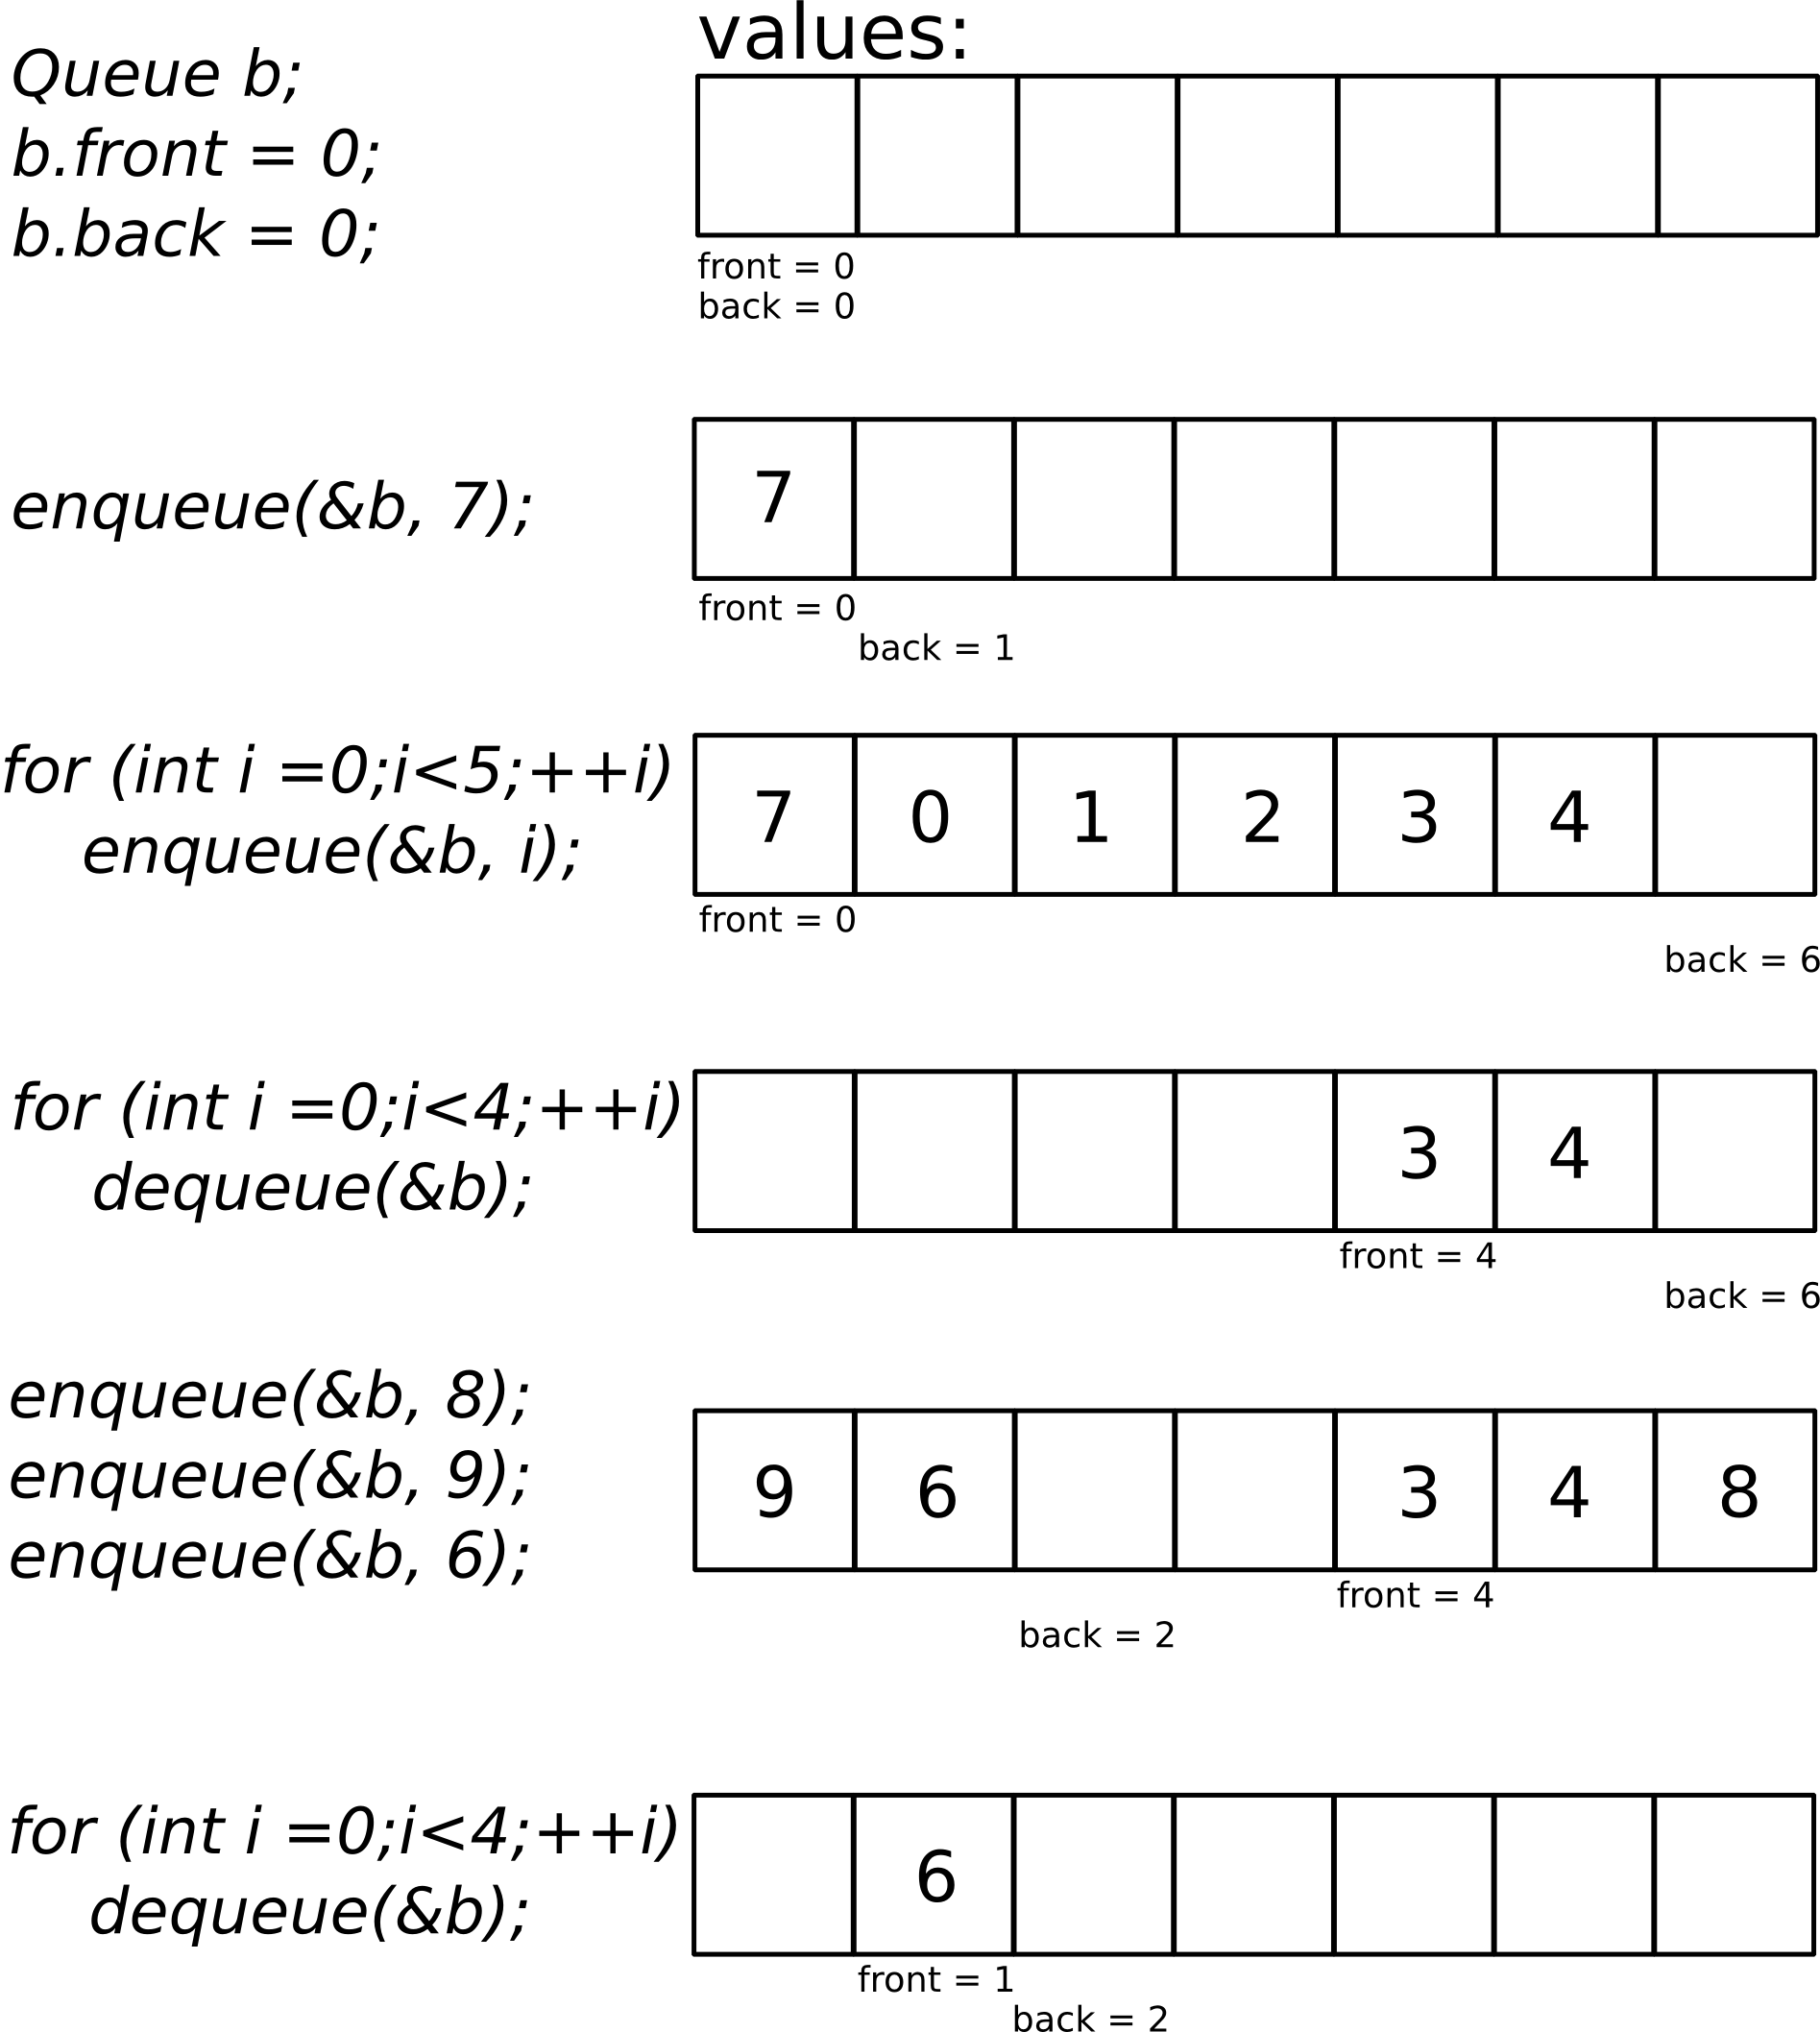
\includegraphics[width=1.05\linewidth]{../images/queue.png}
\end{center}
\end{multicols}

\textbf{Задача \#3: Очередь на основе статического массива}:
\begin{enumerate}
\item Написать функцию \texttt{void queue\_init(Queue* q)}, которая будет задавать начальные значения полей \texttt{front} и \texttt{back}.
\item Написать функцию \texttt{void enqueue(Queue* q, Data x)} - добавляет \texttt{x} в очередь. Для эффективной реализации очереди, нужно использовать как можно меньше операций и как можно эффективней использовать выделенную память. Поэтому, при заполнении массива, если начало массива свободно, то элементы можно хранить там. (смотрите рисунок)
\item Написать функцию \texttt{Data dequeue(Queue* q)} - удаляет элемент из очереди и возвращает его. Для  эффективной реализации очереди сдвигать оставшиеся элементы не нужно. Вместо этого можно просто увеличить поле \texttt{front}.
\item Написать функцию \texttt{int queue\_is\_empty(const Queue* q)}, которая возвращает \texttt{1} если очередь пуста и \texttt{0} иначе.
\item Написать функцию \texttt{int queue\_get\_size(const Queue* q)}, которая возвращает количество элементов.
\item Написать функцию \texttt{int queue\_is\_full(const Queue* q)}, которая возвращает \texttt{1} если очередь заполнена и \texttt{0} иначе. Очередь считается полной, если \texttt{size == capacity - 1}.
\item Написать функции \texttt{Data queue\_get\_front(const Queue* q)} и \texttt{Data queue\_get\_back(const Queue* q)}, которые возвращают элементы, находящиеся в начале и в конце очереди соответственно, но не изменяют очередь.
\item Написать функцию \texttt{void queue\_print(const Queue* q)}, которая распечатывает все элементы очереди.
\item Что произойдёт, если вызвать \texttt{enqueue} при полной очереди или \texttt{dequeue} при пустой? Обработайте эти ситуации. Программа должна печатать сообщение об ошибке и завершаться с аварийным кодом завершения. Чтобы завершить программу таким образом можно использовать функцию \texttt{exit} из библиотеки \texttt{stdlib.h}.
\newpage
\item Протестируйте очередь на следующих тестах:
\begin{enumerate}
\item В очередь добавляется 4 элемента, затем удаляется 2. Вывести содержимое очереди с помощью \texttt{queue\_print()}
\item В очередь добавляется очень много элементов (больше чем \texttt{CAPACITY}). Программа должна напечатать сообщение об ошибке.
\item В очередь добавляется 3 элемента, затем удаляется 2, затем добавляется очень много элементов (больше чем \texttt{CAPACITY}). Программа должна напечатать сообщение об ошибке.
\item В очередь добавляется 3 элемента, затем удаляется 4. Программа должна напечатать сообщение об ошибке.
\item В очередь добавляется 2 элемента, затем выполняется следующий цикл:
\begin{verbatim}
for (int i = 0; i < 10000; ++i)
{
    enqueue(&a, i);
    dequeue(&a);
}
\end{verbatim}
Вывести содержимое очереди с помощью \texttt{queue\_print()}
\end{enumerate}
\end{enumerate}

\textbf{Задача \#4: Очередь на основе динамического массива}:

Описание такой очереди выглядит следующим образом:
\begin{lstlisting}
struct queue
{
    int capacity;
    int front;
    int back;
    Data* values;
};
typedef struct queue Queue;
\end{lstlisting}

\begin{enumerate}
\item Скопируйте код очереди со статическим массивом в новый файл и измените описание структуры как показано выше. Макрос \texttt{CAPACITY} больше не нужен, его можно удалить.

\item Измените функцию \texttt{void queue\_init(Queue* q)} на \texttt{void queue\_init(Queue* q, int initial\_capacity)}. Теперь она должна присваивать \texttt{capacity} начальное значение \texttt{initial\_capacity} и выделять необходимую память под массив \texttt{values}.

\item Измените функцию \texttt{void enqueue(Queue* q)}. Теперь, при заполнении очереди должно происходить перевыделение памяти с помощью функции \texttt{realloc}. Заполнение очереди достигается когда размер очереди становится равным \texttt{capacity - 1} (а не \texttt{capacity}, потому что при полном заполнении вместимости \texttt{front} будет равняться \texttt{back} и мы не сможем понять полная эта очередь или пустая).
После перевыделения нужно переместить элементы массива на новые места и изменить \texttt{front} и \texttt{back}. Если \texttt{front != 0}, то нужно переместить элементы массива от \texttt{front} до конца старого массива \texttt{values} в конец нового массива \texttt{values}. (смотрите рисунок ниже)

\item Добавьте функцию \texttt{void queue\_destroy(Queue* q)}, которая будет освобождать память, выделенную под массив \texttt{values}.

\item Протестируйте очередь: в очередь добавляется много элементов ($\gg 10^3 >$ \texttt{initial\_capacity}). Программа \textbf{не} должна напечатать сообщение об ошибке (если только совокупный размер элементов не превышает размер доступной оперативной памяти). 

\item В случае, если \texttt{malloc} или \texttt{realloc} не смогли выделить запрашиваемый объём памяти (например, по причине того, что этот объём  больше, чем вся доступная оперативная память или по какой-нибудь иной причине), то они возвращают значение \texttt{NULL}. Программа должна это учитывать и завершаться с ошибкой, если нельзя выделить нужный объём памяти.
\end{enumerate}

\subsection*{Схема певыделения памяти для очереди на основе динамического массива:}
Очередь будет считаться заполненной: 
\begin{itemize}
\item Если \texttt{front == 0}, а \texttt{back == capacity - 1}
\item Или если \texttt{front != 0}, а \texttt{front - back == 1}. (А не \texttt{front - back == 0}, потому что при полном заполнении вместимости \texttt{front} будет равняться \texttt{back} и мы не сможем понять полная эта очередь или пустая).
\end{itemize}
 Когда очередь заполнена и мы хотим добавить в неё ещё один элемент, то её нужно увеличить. Делается это так, как представлено на схеме ниже:
\begin{center}
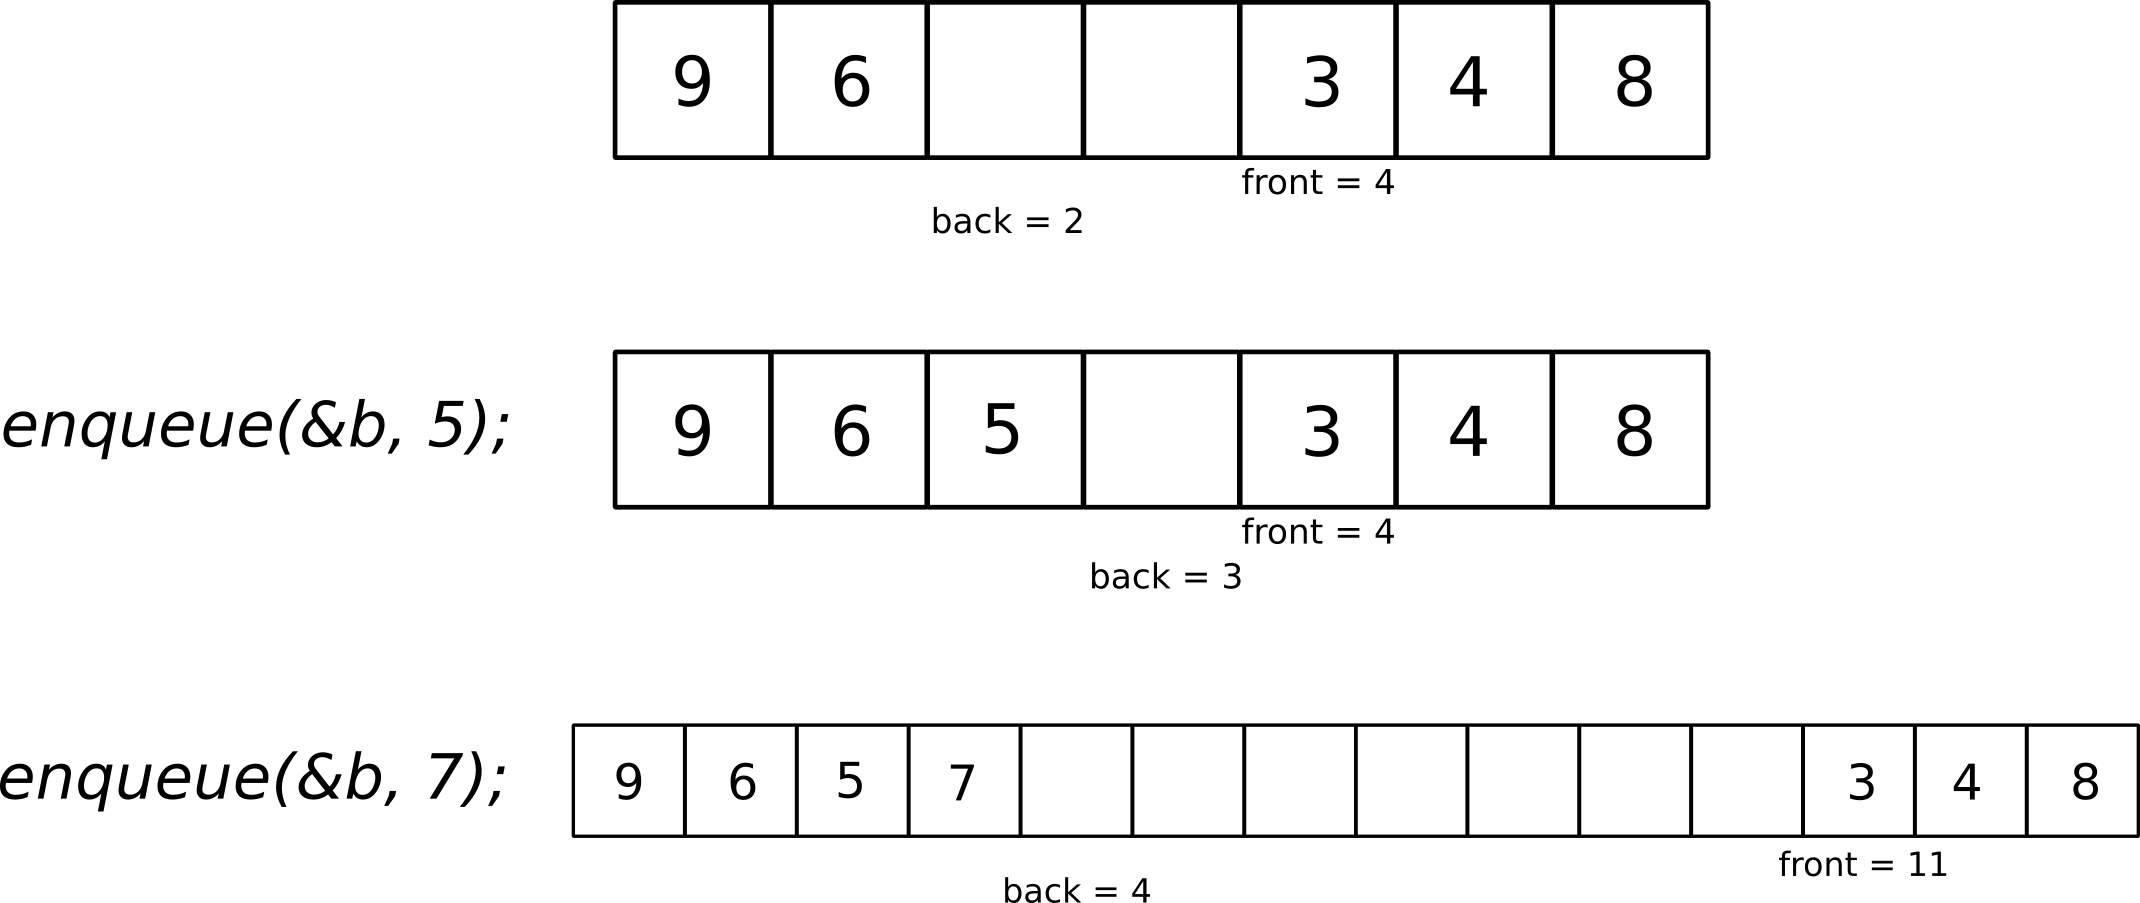
\includegraphics[scale=0.8]{../images/queue_dynamic.png}
\end{center}

\begin{itemize}
\item Если \texttt{front == 0}, то нужно просто увеличить очередь с помощью \texttt{realloc}.
\item Если \texttt{front != 0}, то нужно ещё и перекопировать хвост очереди в конец и изменить \texttt{front}.
\end{itemize}
\end{document}